
\graphicspath{ {\curdir/Graphics/}  }

Hopefully, I have convinced you by now that trapped ions offer the potential to realize the building blocks of a quantum computer.  The difficulty in performing useful quantum computing tasks with them is then relatively easily reduced to the problem of having a sufficient number of communicating qubits available.  A single ion trap can easily confine ten ions, but as more ions are loaded into the trap difficulties begin to arise.  It becomes increasingly difficult to form stable linear chains, and once crystallized, it is more difficult to spatially address individual ions with lasers and to frequency address individual motional modes of the ions.  The motional modes become closer together in frequency and the motional amplitude per ion in each mode is reduced.  Also, the additional motional modes of the trap contribute to decoherence through off-resonant processes.  In order to build an ion trap quantum computer of useful size we will need to couple ions in separate, modular traps.

\section{MUSIQC Architecture}
\label{sec:arch}

To address these issues, a collaboration of ion trappers proposed a new architecture that works towards scalability in two ways. The architecture is known as the Modular Universal Scalable Ion-trap Quantum Computer (MUSIQC) \cite{Monroe:14}.  The first increase in scalability is to implement additional voltage degrees of freedom to improve our control of dc electric fields in ion traps.   In Figure~\ref{fig:musiqc}, this idea is represented by the many small dc electrodes near the trapped ions in the left panel.  This technology will enable us to trap additional ions in a single trapping region and to form additional trapping regions in each vacuum chamber.  In order to easily address and image ions from outside of the vacuum chamber, it is far preferable to crystallize them in a linear chain.  Therefore, their axial confining strength must be kept weaker than their radial confining strength.  The difficulty that arises is that as more ions are loaded into the same trap, the ions at the outer ends of the chain provide additional axial confinement to the center ions through Coulomb repulsion.  The result of which is that trapping increasing numbers of ions in a linear chain requires increasing amounts of radial trap strength to counteract the additional axial confinement.  Especially for heavier ions species, increasing radial strength can become difficult quickly.

\begin{figure}
	\centering
	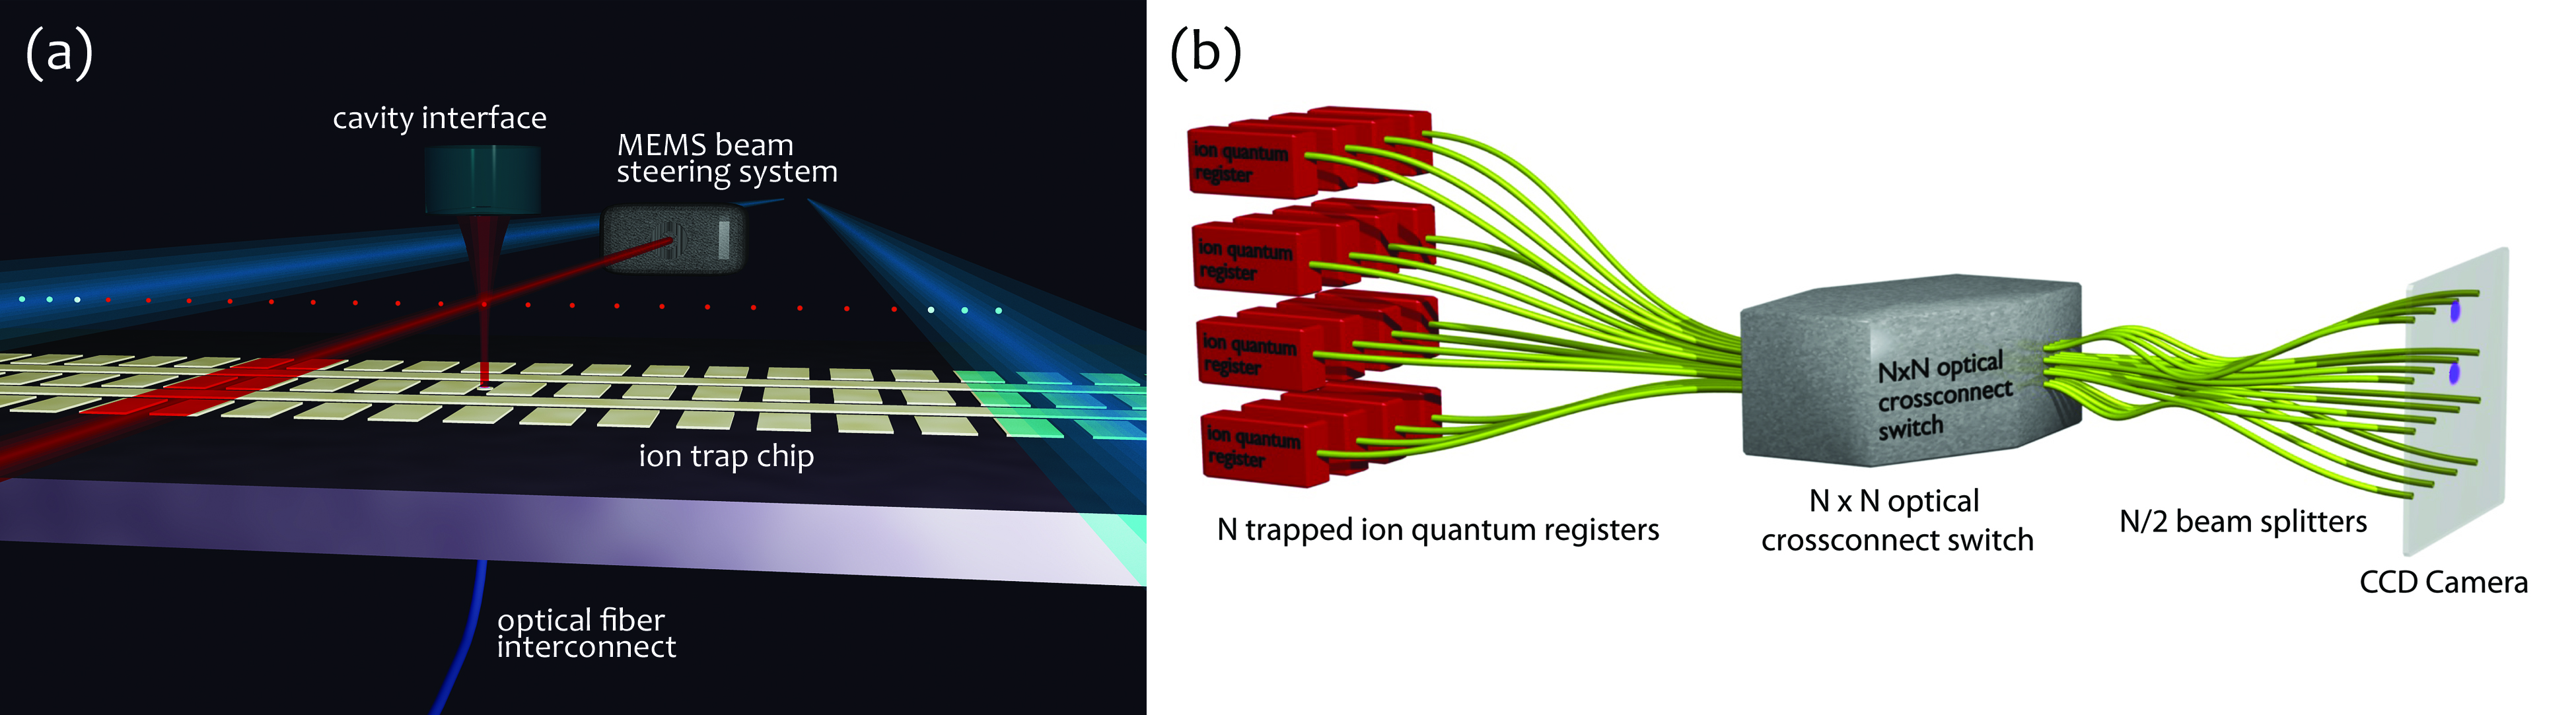
\includegraphics[width=\textwidth]{MUSIQC-plan}
	\caption[Schematic diagram of the MUSIQC architecture]{Schematic diagram of the Modular Universal Scalable Ion-trap Quantum Computer architecture.  Two species of ions are trapped in a surface ion trap with some ions coupled to optical fiber (left).  Photons in these optical fibers can be switched and interfered to generate entanglement between separate modular ion trapping systems (right).}
	\label{fig:musiqc}
\end{figure}

In order to correct for this effect, it is desirable to lower the axial confinement that the center ions experience without compromising the confinement of the entire chain.  Adding higher order anharmonic terms to the axial trap potential can reduce the increase in the axial frequency and allow more ions to be stably trapped \cite{Lin:09}.  Since ions are very sensitive to electric fields, it is easy to add additional controls to their axial potential just by adding more dc control electrodes.  In order to have many small control electrodes, ion traps that are made using standard microfabrication techniques have been developed.  These techniques have been used in the condensed matter community for decades and transfer very well to the manufacture of small ion traps.  Using these additional trap degrees of freedom we expect to be able to trap $\approx$ 20 ions in a trapping region.

Using these additional dc voltage controls, it is also possible to generate and control multiple trapping regions inside the same vacuum chamber.  In fact, generating multiple trapping locations has already been demonstrated, as well as separating ions from and merging ions into these traps \cite{Moehring:11}.  While entangling operations rely on shared motional modes between the ions and can only occur between ions in the same trapping region, entangled ions can be moved between different trapping regions without decoherence \cite{Bowler:12}.  Using these capabilities we can perform our entangling operations in traps with fewer ions and therefore fewer motional modes to improve fidelity and then shuttle the ions back to other trapping locations.  The current usefulness of this procedure is limited by a few concerns.  The separation and merging operations using our current dc control systems take several milliseconds, and the operation might be complicated depending on how many ions need to be reordered to transfer the desired information.  However, with more complicated trap geometries this idea may become more feasible in the future.

Using current surface trap designs, it is possible to store hundreds of ions inside a single vacuum chamber.  While this would be a very impressive technical demonstration, it would not be a modular system and additional scalability would be difficult.  Also, adding more trapping regions to each vacuum chamber increases the difficulty of shuttling ions between them.  All of the lasers applied to the ions need to be carefully focused and directed to avoid interacting with the many other ions inside the $\approx$ 5~mm diameter microfabricated trap.  Applying rf and microwave control fields to single ions in such systems would be very difficult because of their wavelengths, which is unfortunate because many desirable qubit levels are separated by these frequencies.   While none of these difficulties are insurmountable, a separate method of scaling our system will almost certainly prove useful.

The second way that we propose to work towards scalability is by transferring entanglement between separate microfabricated traps or even separate vacuum chambers.  Given an appropriate choice of qubit, it is very easy to generate entanglement between the qubit levels in a trapped ion and single photons \cite{Moehring:04,Stute:12}.  The resulting qubit state of an ion emitting a photon can be encoded into the frequency and polarization of the emitted photon.  The problem of coupling quantum information in ions between vacuum chambers is then reduced to the problem of coupling photons between the chambers.

Coupling photons together is a problem that has already been almost entirely solved.  Optical fiber technology is available that will transfer photons from ions with reasonable loss rates.  Any necessary operations on the photons polarization can be accomplished using optical fiber tools.  The only remaining difficulty is interconnecting the fibers of any desired pair of ion traps.  This last task can be accomplished using a custom microelectromechanical system (MEMS) of mirrors to redirect light from an input array of fibers to any desired output fibers which has already been demonstrated \cite{Olkhovets:04}.  The trapping and quantum operations apparatus can be built into a modular device, and more qubits can be connected by the system by connecting their fiber ports to the fiber switch (see the right panel of Figure~\ref{fig:musiqc}).

For reasons discussed in the next section, this photonic information transfer will be significantly slower than the timescale of other operations in the trap.  Quantum gates between ions in the same trap can usually be performed at rates of $\approx$ 100~kHz to 1~MHz.  Shuttling ions containing information between separate trapping regions can be accomplished at a rate of $\approx$ 1~kHz - 10~kHz.  Transferring quantum information between remote ions in separate vacuum chambers can currently be done at 1~Hz to 10~Hz, but we believe that we can increase this rate to $\approx$ 1~kHz.  Nevertheless, quantum algorithms will be possible using this architecture. Analysis has shown that the MUSIQC architecture compares favorably with other commonly suggested scalable quantum computer architectures \cite{Monroe:14}.  The slower remote entanglement step also does not preclude the implementation of quantum error correction.

\section{Remote Entanglement}
\label{sec:remote}

The first step to implementing this remote ion-ion entanglement procedure is collecting single photons from trapped ions.  Each modular trap system will need to feature one or more locations that are optically coupled to a single mode optical fiber.  An ion trap system that was not designed with this feature in mind will usually collect approximately 2\% of the available ion fluorescence using a long working distance microscope objective placed outside of the vacuum chamber.  The resulting probability of successfully managing to entangle two ions in distant traps in a single trial will be very small.  Attempting the entanglement and hoping that it worked is not a realistic possibility.  Fortunately, there is a protocol by which it can be determined whether the entanglement process was successful without performing a measurement that would destroy the entanglement.

First, we must simultaneously couple two single photons each entangled with an ion in separate modules.  The ion is initialized to one qubit state and then excited to a state that can decay to either qubit state by emitting a distinguishable photon (see Figure~\ref{fig:remoteentangle}).  For example, considering vacuum chambers $A$ and $B$, photon quantum states $\ket{H}$ and $\ket{V}$, and ion qubit states $\ket{\uparrow}$ and $\ket{\downarrow}$ we will generate the state
\begin{equation}
	\ket{\Psi} = \bigotimes_{i=A,B} \frac{1}{\sqrt{2}} \left( \ket{H}_{i}\ket{\uparrow}_{i} + \ket{V}_{i}\ket{\downarrow}_{i} \right)\mathrm{.}
\end{equation}
The photon states need to be some distinguishable photon states maximally entangled with the ion states.  Polarization states can be used easily or frequency states can be used if the frequency separation is larger than the linewidth of the transition.  We can then overlap the photon spatial modes on a 50-50 beamsplitter at some other location.  When single photon detectors placed at both output ports of the beamsplitter are simultaneously triggered that will correspond to measuring the photon state as $\frac{1}{\sqrt{2}} \left( \ket{H}_A\ket{V}_B - \ket{V}_A\ket{H}_B \right)$.  If the photons were both in $\ket{H}$ or both in $\ket{V}$, the probabilities of both photons reflecting off the beamsplitter or both transmitting through the beamsplitter interfere and the photons must both be output on the same interferometer arm.  We can determine the resulting state of the ion by projecting the measured photon state onto $\ket{\Psi}$.  The ions are left in the state
\begin{equation}
	\ket{\Psi}_\mathrm{ion} = \frac{1}{\sqrt{2}} \left( \ket{\uparrow}_A \ket{\downarrow}_B - \ket{\downarrow}_A \ket{\uparrow}_B \right)
\end{equation}
which is a maximally entangled state of the ion qubits.  This procedure destroys the initial qubit state of the ions, but remotely entangled qubits can be prepared in advance and used a resource during the computation.

\begin{figure}
	\centering
	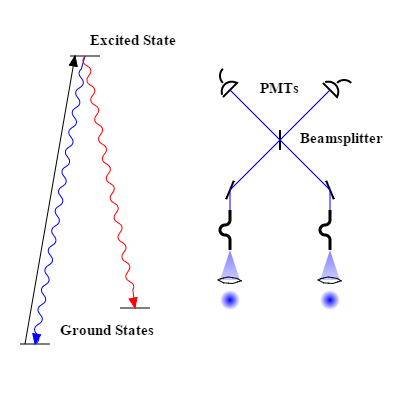
\includegraphics[width=0.6\textwidth]{remote-entanglement}
	\caption[Remote ion-ion entanglement procedure]{Diagram of the remote ion-ion entanglement experiment.  An ion is excited to a state with two possible photon decay paths (left).  The photons are collected and interfered before being detected on two PMTs (right).  The overlap of the spatial modes removes the which-path information from the system before the detection and leaves the ions entangled.}
	\label{fig:remoteentangle}
\end{figure}

Successful remote ion-ion entanglement in small scale systems with other ion species has been successfully demonstrated \cite{Matsukevich:08}.  We have begun generating entangled ion-photon pairs and are working towards a remote ion-ion entanglement demonstration using barium ions \cite{Auchter:14}.  In any given attempt an entangled ion-photon pair can be generated with probability $P$ given by,
\begin{equation}
	P = P_\mathrm{exc} f  \eta \frac{\Omega}{4 \pi} f_\mathrm{gate} T
\end{equation}
where $P_\mathrm{exc}$ is the probability of driving the transition to the excited state ($\approx$ 0.2 in our current experimental setup), $f$ is the branching ratio back to the initial state if other decays are possible ($\approx$ 0.75), $\eta$ is the quantum efficiency of the single photon detector ($\approx$ 0.2), $\Omega$ is the solid angle for the collection optics ($\approx 0.02 \times 4 \pi$), $f_\mathrm{gate}$ is the fraction of emitted photons in our detection window ($\approx$ 0.8), and $T$ accounts for other losses including transmission through all other optics ($\approx$ 0.3).  These factors currently limit us to generating an entangled ion-photon pair at about 2.5~Hz given our 17~kHz repetition rate \cite{Auchter:14}.  

Generating an entangled ion-ion pair requires the simultaneous generation of two ion-photon pairs which means that it only succeeds with probably proportional to $P^2$.  The photons must also be transmitted through a length of optical fiber, have their spatial modes overlapped, and be in a correct state to allow the heralded entanglement scheme to occur, but these factors are insignificant or unavoidable.  The largest achievable gains in our apparatus would be to $P_\mathrm{exc}$ which can easily be increased to unity, and $\Omega$ which can be increased by a factor of 5 to 10.  The MUSIQC collaborators are exploring a number of possible methods to improve $\Omega$ including in vacuum cavities \cite{Sterk:12} and diffractive optics \cite{Clark:14}.  We have designed and built an ion trap inside of a parabolic mirror which can be used to collect $\ge 40\%$ of an ion's fluorescence \cite{Shu:11}, and we are working to implement ion-ion entanglement experiments in that system.  Using currently available technology, we believe a remote ion-ion entanglement rate of $\approx$ 1~kHz is feasible and we are working towards achieving that goal.

\section{Mixed Ion Species}
\label{sec:mixed}

Unfortunately, as the implementation of this scheme proceeded, field crosstalk between neighboring ions was a problematic issue.  The generation of remote entangled ion pairs requires the application of resonant laser beams on strong transitions.  Even with ion separations of 10~microns, well focused lasers can still scatter hundreds of photons per second from neighboring ions.  Scattering any photon will completely destroy the quantum information that might have previously been held in the ion, and can quickly disrupt an entire calculation.  The determination was eventually made that we needed to take measures to avoid this problem.

\begin{figure}
	\centering
	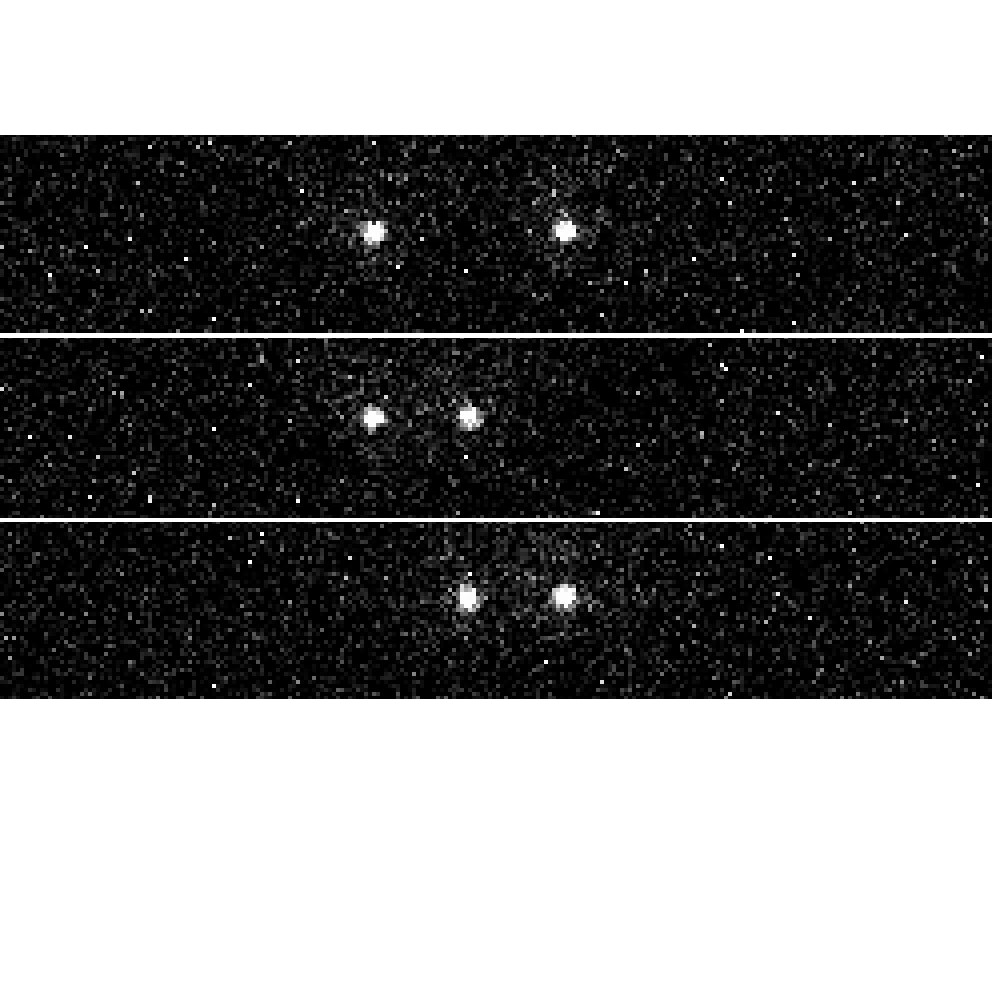
\includegraphics[width=0.6\textwidth]{BaYb}
	\caption[CCD image of barium and ytterbium ions]{CCD image of two barium and a ytterbium ion in the a linear ion crystal.  Fluorescence from the barium ions is visible, while the ytterbium ion is dark.  The ytterbium ion is in the center in the top panel, the left in the middle panel, and the right in the bottom panel.}
	\label{fig:bayb-ccd}
\end{figure}

The method chosen to minimize the field crosstalk issue was to use separate ion species for quantum computation and the remote entanglement generation.  This choice cements the idea of remote entangled pairs as a computational resource.  One ion species can be dedicated to generating many entangled pairs that can be transferred into the computation by quantum teleportation of the entanglement onto the computational ion species.  Only the computational ion species will store quantum information for any significant period of time or perform any calculations with it.  Previous work towards a similar mixed ion species system has been done with small numbers of ions already \cite{Lin:13}.

Another advantage of adopting this scheme is that there are now many ions motionally coupled to the computational ions, but with well-separated optical transition frequencies.  Laser cooling can be performed on the remote entanglement species with a negligible chance of scattering a photon from the computational ions.  Since the two species are motionally coupled, it should be possible to keep the entire chain of ions cold without affecting ongoing quantum algorithms.  By using quantum gates that are insensitive to small motional occupation numbers and electromagnetically-induced-transparency cooling \cite{Lin:13, Roos:00}, it may even be possible to avoid ever having to laser cool the computational ions.  This would allow quantum algorithms to continue running until qubit begins to decohere instead of being forced to stop by heating issues as is often the case.  The use of the M{\o}lmer-S{\o}rensen gate discussed in Chapter~\ref{sec:qcomp} is also helpful here because of its resistance to decoherence even when performed at finite ion temperatures and during ion heating.  

The added difficulty in only laser cooling one species is that different ion species obviously have different masses, which causes each normal mode of the chain to couple more strongly to one ion species than the other.  For large mass differences, this imbalance can make it impossible to cool one ion species using the other.  Each mode will have eigenvector components of order one with one ion species and all of its eigenvector components with the other ion species may be $\le$ 0.01 or even less.  The result is that even with large amounts of energy in this mode, the ion species being laser cooled may have very little motion.  

It is hoped that by choosing ion species with small mass differences and by exploring other degrees of freedom, this cooling scheme may be possible.  These other degrees of freedom include number and arrangement of the cooling ions and overall trap strengths and anharmonicities.  After going through our ion trapping, cooling, initialization, and readout procedures in more detail in Chapters~\ref{sec:trap} and \ref{sec:ioncool}, I will explore these ideas further.

The two ion species that will be used for the MUSIQC program are ytterbium and barium.  We have already successfully trapped these two species in the same linear ion chain (see Figure~\ref{fig:bayb-ccd}).  Ytterbium-171 has a pair of ground state levels with excellent insensitivity to magnetic fields.  These levels have very long coherence times and the state of the ion can be determined using a simple optical setup.  Barium has the advantage of having a strong transition at 493~nm, which is a long wavelength transition among ion species that can be laser cooled.  This wavelength is transmitted through fibers easier than more ultraviolet transitions which will improve the rate at which remote entangled pairs can be generated.  Further the two species are relatively close in mass, which should help to improve their motional coupling.

